% El uso del trazado de rayos como aproximación a ondas electromagnéticas no es una idea reciente, aunque su alto coste computacional ha hecho que su popularidad haya crecido de forma notable en los últimos años al haber sido posible su uso de forma general.

% La principal disciplina en busca de implantaciones de esta técnica es la de gráficos generados computacionalmente, en la que se aplican estas aproximaciones a la luz de modo que se puedan conseguir resultados realistas de una forma más sencilla comparado con la rasterización habitual en la industria.

% Encontramos en la bibliografía de este ámbito numerosos capítulos dedicados a la implantación del trazado de rayos que han sido recuperados en este trabajo.
% Aunque las bases geométricas son similares, las características electromagnéticas de los rayos de luz simplifican parte de los cálculos que debemos corregir en nuestro caso.

La proliferación del uso de ondas electromagnéticas como sustitución de conexiones cableadas ha aumentado su uso de forma significativa en las últimas décadas, especialmente entornos interiores.

Determinar la propagación de este tipo de ondas en estos escenarios resulta una parte fundamental en el estudio de su rendimiento y abre la puerta a aplicaciones adicionales además de la comunicación, como pueden ser algoritmos de posicionamiento en interiores.

De forma teórica existen técnicas de resolución de ecuaciones diferenciales aplicadas al campo electromagnético como el FDTD --\textit{Finite-difference time-domain method}--, especialmente modificadas para adaptarse a la relación entre campos eléctrico y magnético.\cite{Compilation}

Este tipo de métodos numéricos, aunque precisos, requieren un alto coste computacional.
Estan planteados como métodos generales, aplicables a cualquier tipo de onda electromagnética por lo que se pueden tomar aproximaciones que relajen los requisitos.

Teniendo en cuenta que las ondas a tratar en comunicaciones están en un régimen de alta frecuencia aparecen métodos que aproximan las ondas a rayos unidimensionales que se propagan en el espacio interactuando con todo tipo de objetos.

\subsection{Aproximación de la emisión electromagnética a rayos}

La aproximación de la emisión de ondas como propagación de rayos resulta una idea intuitiva ya explorada en otros ámbitos de la física relacionados con propagación de ondas como pueden ser fenómenos sismológicos o acústicos.

Dentro del ámbito de campos electromagnéticos, esta aproximación ha sido tradicionalmente usada en la óptica geométrica en aplicaciones como diseño de lentes o espejos.

En el caso de ondas electromagnéticas de forma general --más allá del ejemplo anterior de ondas de luz--, su uso principal es el de la propagación de ondas de radio.
La proliferación de su uso desde el siglo pasado ha requerido técnicas de análisis para la arquitectura de sistemas de comunicación inalámbricos, de modo que sea posible determinar el camino seguido por las ondas de radio y tener comunicaciones fiables en condiciones sin visión directa.

Los primeros estudios aparecen en la estregia para aprovechar la capa de la ionosfera de la atmósfera para la comunicación entre puntos de la Tierra sin visión directa por la geometría esférica.

En estos casos los distintos índices de refracción modificarán la trayectoria antes y después de los rebotes buscados complicando la predicción del camino seguido de forma general.
Por ello, se usa la aproximación de rayos para determinar las posiciones de los receptores y los ángulos de emisión requeridos.

La misma estrategia es seguida en propagación de ondas de telefonía móvil.
En este caso el problema a resolver es comprobar las zonas con una mayor atenuación en zonas con una alta densidad urbanística, de modo que sea posible colocar emisores en posiciones óptimas de modo que estas zonas tengan el menor área posible.

En este trabajo se retoma esta aproximación en un entorno local.
La estrategia de emisión de rayos no es escasa en la bibliografía en este ámbito: al igual que en los casos expuestos anteriormente, la parametrización a priori de los obstáculos en la propagación hace prácticamente imposible aplicar métodos analíticos o estadísticos para evaluar de forma fiable la recepción de las ondas emitidas.

La correcta determinación de la propagación en entornos controlados habilita la predicción con una alta precisión del rendimiento de los receptores en cualquier zona del mismo, lo que permite no solo una correcta colocación de los mismos --en caso de que se quiera garantizar una correcta recepción en cualquier zona-- si no que abre la puerta a posibles aplicaciones como las de posicionamiento local.

La alternativa a la simulación de esta propagación es la medición sobre el terreno de los valores de la onda, bien eligiendo ciertos puntos de forma homogénea o buscando lugares concretos de interés.
Esta técnica, conocida como \textit{fingerprinting}, es muy lenta y obliga a desplazarse a la zona de interés, por lo que la opción de realizar una simulación presenta una gran ventaja a la hora de ahorrar tiempo y costes, además de permitir una precisón mayor pudiendo obtener los valores de recepción en cualquier punto de la zona a medir.\cite{People}

La aproximación de ondas electromagnéticas a rayos proviene del concepto de frente de ondas, en el que se considera un cierto plano de propagación de las ondas.
Según las ecuaciones de Maxwell los campos eléctrico y magnético son perpendicualares a este frente, y con ellos aparece el vector de Poynting.\cite{Compilation}

Este vector, definido como el producto vectorial de ambos campos, contiene en su módulo la potencia de la onda --tomando medias temporales--, y en su dirección la dirección de propagación.
En ausencia de cambios en el índice de refracción del medio --es decir, en medios homogéneos--, la dirección del frente de ondas y del vector de Poyinting no se modificará, así que la onda seguirá su trayectoria en línea recta.

Es este vector el utilizado para modelizar los rayos, de modo que cumplen tres características:
\begin{itemize}
    \item Los rayos se transmitirán en línea recta en un medio homogéneo.
    \item Los rayos contienen información sobre la potencia de la onda transmitida.
    \item Los rayos sufrirán fenómenos de reflexión y refracción a su encuentro con los obstáculos del medio.
\end{itemize}

\subsubsection{Algoritmos de trazado de rayos}

En general, todos los algoritmos buscarán encontrar la manera de determinar impactos entre los rayos y los obstáculos del entorno, pero existen distintas estrategias para determinar estas colisiones.

\subsubsection*{Divisiones uniformes}

En esta estrategia se busca la división de la zona de interés en cuadrados o cubos de forma unifome.

Con estas divisiones se busca cuál es la posición del rayo en cada momento de modo que se puedan determinar las propiedades buscadas en cada división, pudiendo obtener dichos valores en cada parte del mapa.

Si la geometría de la zona no es regular es posible definir zonas con distintos tamaños y así poder tener zonas con una granularidad mayor.

\subsubsection*{\textit{Bounding box}}

Otra de las técnicas viene heredada de la resolución del problema de colisiones habitualmente usando en videojuegos.

Aquí se busca modelizar los objetos con un cierto volumen, de forma que es posible determinar la existencia de una cierta colisión en caso de que alguno de ellos llegan a compartir cierto espacio.

Para mejorar el rendimiento es común usar una jerarquía de modo que sea posible agrupar los objetos en cajas mayores.
Así, se buscará en primer lugar cuál de estas \textit{bounding boxes} mayores será impactada, y luego iterar sobre sus componentes, eliminando la necesidad de comprobar todos los objetos de la escena y ahorrando coste computacional.

En este caso solo se encontraran estas colisiones entre rayos y obstáculos, pero no se registrará su paso por el espacio libre.
Para ello aparece la idea de usar otros obstáculos como receptores.

El concepto de receptor en este caso no diferirá del del obstáculo en su modelización: será un elemento del mismo tipo, pero no generará rebotes.
En el caso de que un rayo impacte con él, se registrará su potencia al colisionar y se dejará evolucionar al rayo incidente sin modificarlo.

\subsubsection*{Colisiones con mallas}

La modelización de forma habitual de modelaje en tres dimensiones cuando la geometría no es regular consiste en formar un mallado de triángulos.
Siendo una estretegia habitual y ampliamente usada en entornos de diseño, surgen implementaciones que aprovechan este tipo de modelos.

En estos casos la búsqueda de colisiones se produce buscando el punto de intersección entre la recta del rayo y el plano en el que alguno de los triángulos está contenido, comprobando más tarde sus límites.
También es habitual el uso de coordenadas baricéntricas, que no dependen de la orientación del triángulo en el espacio. \cite{Graficos}

Esta estrategia ha sido la utilizada en esta simulación.
En lugar de triángulos, en este caso se han usado rectángulos, aunque la base es la misma.
En secciones posteriores se abodará la geometría necesaria para estos casos.

Al igual que en el caso del \textit{bounding box}, será necesario colocar receptores en aquellos lugares de interés de modo que sea posible registrar los parámetros necesarios en ciertos puntos del mapa.


\subsection{Geometría del trazado de rayos}

\subsubsection{Rayos}
Los rayos a evaluar son el elemento básico a caracterizar.
Su composición es muy simple: constan de un punto de origen y una dirección.
En su transcurso se encontrarán con las paredes del mapa, contra las que rebotarán para seguir su recorrido en la zona de interés.

Para poder modelizar este comportamiento se considera el rayo como una recta.
En este caso el origen $O$ será un punto de esta recta, con su dirección siendo el vector director $\vb{d}$ de la misma de modo que sigue la ecuación
\begin{equation}
    O + t\vb{d}
\end{equation}
con $t\in \mathbb{R}$.

\subsubsection{Paredes}
\label{sec:paredes}

\begin{wrapfigure}{r}{0.35\textwidth}
    \centering
    \hspace*{0.5cm}
    \def\svgwidth{0.3\textwidth}
    \input{svg/rayo-plano.pdf_tex}
    \caption{Esquema de la intersección entre rayo y plano.}
    \label{fig:rayo_plano}
\end{wrapfigure}
Las paredes serán planos definidos con cuatro puntos como extremos, a partir de los cuáles se calcula su vector normal.
Así, los puntos de intersección de las rectas con alguno de estos planos serán los puntos donde los rayos golpearán las paredes, que servirán de origen para los rayos trasmitidos y reflejados que se generen.

Para determinar cuál es este punto de impacto partimos de la consideración de que el vector normal del plano --denominado aquí $\vu{n}$-- será perpendicular a cualquier vector contenido en dicho plano, en este caso el definido como diferencia entre el punto de intersección $X$ y el punto donde está definida la normal\footnote{Esta consideración proviene del caso de una superficie general; en este caso la normal será la misma independientemente de dónde se defina, pudiendo elegir cualquier punto del plano.} $P$ de tal forma que su producto escalar es nulo
\begin{equation}\label{eq:Plano-recta1}
    (X-P)\vdot\vu{n} = 0
\end{equation}

La Figura~\ref{fig:rayo_plano} contiene un esquema de dicha disposición, donde se puede comprobar la perpendicularidad de este vector.

$X$ es un punto de la recta, por lo que debe cumplir, para un cierto $t_i$
\begin{equation}\label{eq:recta_ti}
    X = O + t_i\vb{d}
\end{equation}
que es posible incluir en \eqref{eq:Plano-recta1} de forma que
\begin{equation}
    ((O + t_i\vb{d})-P)\vdot\vu{n} = 0
\end{equation}
que se puede manipular para obtener $t_i$
\begin{equation}\label{eq:t_i}
    \begin{aligned}
        ((O + t_i\vb{d})-P)\vdot\vu{n} &= 0 \\
        (O - P)\vdot\vu{n} + t_i\vb{d}\vdot\vu{n}  &= 0 \\
        t_i\vb{d}\vdot\vu{n} &= - (O - P)\vdot\vu{n}\\
        t_i &= -\frac{(O - P)\vdot\vu{n}}{\vb{d}\vdot\vu{n}}\\
        t_i &= \frac{(P-O)\vdot\vu{n}}{\vb{d}\vdot\vu{n}}
    \end{aligned}
\end{equation}

Con este valor es posible ahora usar la Ec.~\eqref{eq:recta_ti} para obtener las coordenadas del punto de impacto, pero no en cualquier caso.

Es necesario tener varias consideraciones a la hora de determinar $t_i$.
La primera de ellas es que es posible obtener un valor negativo: al modelizar el rayo como una recta se abre la posibilidad de encontrar un punto de intersección en la dirección contraria al vector director, por lo que consideraremos que no hay intersección si $t_i < 0$.

Otra de las posibilidades es que la recta sea paralela al plano, de tal forma que no exista un punto de intersección.
Si esto ocurre, el producto escalar del denominador de la Ec.~\eqref{eq:t_i} tomará un valor nulo, por lo que es necesario evitar la operación.

Es más, es posible optimizar este caso en un grado algo mayor al tener en cuenta que ángulos bajos de la normal del vector y la dirección de la recta también indicarán que la intersección se producirá a una distancia muy lejana, por lo que a efectos prácticos no se producirá --habrá otra pared más cerca--.
Así, en el caso de que $\vb{d}\vdot\vu{n} < 10^{-4}$ se interpretará que no hay un punto de intersección con la pared a evaluar.

La última de las consideraciones tiene que ver con los errores de redondeo.
A la hora de calcular $t_i$ o las coordenadas del punto de impacto es posible que el punto de intersección obtenido no se encuentre en el plano de incidencia, lo que provoca futuros errores con los rayos reflejados y transmitidos.
Para evitarlo, solo se considerará la intersección con los planos si $t_i > 10^{-3}$.

\begin{figure}[H]
    \centering
    % Primera version
% \begin{tikzpicture}
%     %Pared
%     \draw[thick] (-6,0) -- (-2,0);

%     \draw[-Triangle] (-6,1.5) -- (-4.5,0);
%     \draw[-Triangle, dashed] (-4.5,0) -- (-3.5,-1);

%     \draw (-4.5,0) circle [radius=2pt];
%     \filldraw (-3.5,-1) circle [radius=2pt, fill=black];

%     % Flecha del medio.
%     \draw[-{Triangle[width=18pt,length=8pt]}, line width=10pt] (-0.5,1) -- (0.5, 1);

%     % Segunda parte
%     %Pared
%     \draw[thick] (2,0) -- (6,0);

%     \draw (2.5,0) circle [radius=2pt];
%     \draw[-Triangle] (2.5,0) -- (4,1.5);

%     \filldraw (3.5,-1) circle [radius=2pt, fill=black];
%     \draw[-Triangle, dashed] (3.5,-1) -- (4.5,0);
% \end{tikzpicture}

% Segunda version.
\begin{tikzpicture}
    %Pared
    \draw[very thick] (-5,0) -- (5,0);

    \draw[-Stealth] (-3.5,2) -- (-2.5,1);
    \draw (-2.5,1) -- (-1.5,0);
    \draw[-Stealth, dashed] (-1.5,0) -- (-0.5,-1);

    \draw (-1.5,0) circle [radius=3pt];
    \filldraw (-0.5,-1) circle [radius=3pt, fill=black];

    \draw[-Stealth] (-1.5,0) -- (0.5,2);
    \draw[dashed, -Stealth] (-0.5,-1) -- (0,-0.5);
    \draw[dashed, -Stealth] (0,-0.5) -- (0.5,0);

    \filldraw (0.5,0) circle [radius=3pt, fill=black];
\end{tikzpicture}
    \caption{Puntos de intersección en presencia de errores de redondeo: al estar fuera del plano, la evaluación del rayo reflejado encuentra otro punto de intersección en la misma pared. Los círculos huecos y líneas sólidas indican los puntos y rayos correctos; los círculos rellenos y líneas punteadas representan los puntos y rayos calculados erróneamente.}
    \label{fig:condicion_interseccion}
\end{figure}

Esta condición puede parecer confusa pero su razón se puede ver en la Figura~\ref{fig:condicion_interseccion}.
Debido a errores de redondeo, los rayos reflejados y transmitidos no tienen su origen en el plano de incidencia, por lo que al evaluarlos, encontraremos que la pared con la que impactaría sería, de nuevo, el mismo plano.

Con la condición introducida, no habrá intersecciones estos planos tan cercanos, por lo que el rayo será libre de obviarlo y buscar un rebote en alguna otra pared, como debería haber hecho sin los errores de redondeo.

Aunque en este ejemplo solo se han representado los rayos reflejados, en el caso de que el punto de intersección se encuentre --de nuevo, siguiendo la simetría del ejemplo-- delante del plano tendríamos la misma situación al evaluar el rayo transmitido.

Estos nuevos puntos no solo son erróneos --no se deberían producir--, sino que además pueden llegar a producir valores totalmente distorsionados de la potencia de la señal como se explicará en secciones sucesivas.

Una vez determinado el punto de impacto, es necesaria una última comprobación.
Al igual que al hablar de las rectas se ponía su manifiesto su extensión infinita, es posible tener la misma consideración con los planos, es decir, será posible encontrar puntos de intersección en cualquier punto del espacio.

Para imponer la presencia de los puntos de intersección entre los límites de la pared es necesario recurrir a sus esquinas --los puntos sobre los que se definen--.
Tras determinar el punto de intersección, se comprueba, para cada dimensión, que su coordenada se encuentra entre los valores máximos y mínimos de las coordenadas de la pared en dicha dimensión.

Será necesario añadir un cierto épsilon para, de nuevo, evitar los errores de redondeo, y así evitar que el plano no «sea invisible» al rayo.
Por tanto, la comprobación a realizar será, que para cada dimensión $i$, las coordenadas estén contenidas en $[\min_i(c_{ij})-\varepsilon, \max_i(c_{ij})+\varepsilon]$ siendo $c_{ij}$ la coordenada $i$ de la esquina $j$.

\subsubsection*{Geometría tras los impactos}

Una vez obtenido el punto de impacto del rayo en la pared, queda evaluar los rayos obtenidos a partir de él.

\begin{wrapfigure}{r}{0.3\textwidth}
    \vspace*{-0.75cm}
    \centering
    \begin{tikzpicture}
    %Pared
    \draw[very thick] (0,2.5) -- (0, -2.5);

    \draw[thick, -Stealth] (0,0) -- (-1.5,1.5);
    \draw[thick] (-1.5,1.5) -- (-2,2);
    \node[anchor=west] at (-1.5,1.5) {$\vb{d}_i$};

    \draw[thick, -Stealth] (0,0) -- (-1.5,0);
    \node[anchor=east] at (-1.5,0) {$\vu{n}$};

    \draw[thick, -Stealth] (0,0) -- (-1.5,-1.5);
    \draw[thick] (-1.5,-1.5) -- (-2,-2);
    \node[anchor=west] at (-1.5,-1.5) {$\vb{d}_s$};

\end{tikzpicture}
    \caption{Reflexión especular.}
    \label{fig:reflexion}
\end{wrapfigure}
En cada uno de estos impactos se generá un rayo reflejado y un rayo transmitido.
El rayo reflejado seguirá una reflexión especular, de modo que su dirección seguirá
\begin{equation}
    \label{eq:reflexion}
    \vb{d}_s = 2(\vu{n} \vdot \vb{d}_i)\vu{n} - \vb{d}_i
\end{equation}
donde $\vb{d}_i$ indica la dirección del rayo incidente y $\vb{d}_s$ la del rayo reflejado, ambos vectores normalizados.

La Ec.~\eqref{eq:reflexion} supone la disposición de las direcciones tal y como se indica en la Figura~\ref{fig:reflexion}, de tal forma que ambas se indican partiendo desde la pared.
Desde la perspectiva del rayo incidente, esta dirección será la inversa a su dirección de incidencia.

% En el caso del rayo transmitido, su dirección será la dirección de entrada pues no se considerarán efectos de refracción.
% El material entre las paredes será siempre aire, y teniendo en cuenta que se consideran...

Una vez determinado el rayo reflejado queda evaluar el rayo transmitido.
Para ello se recurre a la ley de Snell para la refracción, pero teniendo en cuenta que estamos considerando las paredes como planos bidimiensionales, los rayos transmitidos compartirán la dirección del rayo impactado.

\begin{figure}[H]
    \centering
    \begin{tikzpicture}
        \draw[dashed] (-4.5,0) -- (0,0);
        \draw[dashed] (0,1) -- (4.5,1);
        
        \draw[thick] (-2,-1.5) -- (-2, 3);
        \draw[thick] (2,-1.5) -- (2, 3);

        % Rayos
        \draw[->] (2,1) -- (4,3);
        \draw[->] (-4,-2) -- (-2,0);
        \draw[->] (-2,0) -- (2,1);

        %Ángulos
        \draw[thick] (-3,0) arc(180:225:1);
        \node[anchor=east] at (-3,-0.5) {$\theta_1$};
        
        \draw[thick] (-1,0) arc(0:15:1);
        \node[anchor=west] at (-0.5, 0.15) {$\theta_2$};

        \draw[thick] (3,1) arc(0:45:1);
        \node[anchor=west] at (3, 1.5) {$\theta_3$};



        % Labels
        \node[anchor=south] at (-3.5,-2.5) {$n_1$};
        \node[anchor=south] at (0,-2.5) {$n_2$};
        \node[anchor=south] at (3.5,-2.5) {$n_3$};
    \end{tikzpicture}
    \caption{Rayos refractados al atravesar un material considerando un cambio de medio.}
    \label{fig:snell_plano}
\end{figure}

Al igual que la dirección también tendrán como origen el punto de impacto, debido a la bidimensionalidad del plano.
La Figura~\ref{fig:snell_plano} indica el caso de una pared con un cierto grosor.

Los ángulos de entrada y salida serán los mismos sin más que comprobar la ley de Snell.\cite{Graficos}
Para el primer borde
\begin{equation}
    n_1\sin(\theta_1) = n_2\sin(\theta_2)
\end{equation}
y para el segundo, si el último medio fuese distinto
\begin{equation}
    n_2\sin(\theta_2) = n_3\sin(\theta_3)
\end{equation}

Teniendo en cuenta que $n_1=n_3$, está claro que $\sin(\theta_1)=\sin(\theta_3)$, por lo que ambos ángulos tomarán el mismo valor y sus direcciones serán las mismas.

En cuando al punto de origen del nuevo rayo, ya en la Figura~\ref{fig:snell_plano} se puede observar que vendrá determinado por el ángulo $\theta_2$ y el tamaño de la pared.
En el caso en el que este tamaño sea cero, el desplazamiento también lo será, por lo que el origen del nuevo rayo será el punto de impacto.

\subsubsection*{Determinación del ángulo de impacto}

Como se explica en siguientes secciones, será necesario evaluar el ángulo de impacto del rayo en la pared para obtener la potencia de los rayos generados.

Este valor se obtiene sin problema teniendo en cuenta que su coseno será el producto escalar de la normal y el vector de la dirección incidente --más concretamente de su inverso, como se puede observar de nuevo en la Figura~\ref{fig:reflexion}--, pero es necesario hacer una puntualización.

El cálculo de la normal del plano se define a partir de las tres primeras esquinas introducidas para cada pared.
Por ello, dependiendo del orden en el que se escriban será posible que la normal tome un sentido o su opuesto.

En las ecuaciones \eqref{eq:t_i} y \eqref{eq:reflexion} ese cambio de signo es irrelevante, pero no en este caso.
Si la normal está definida en la dirección opuesta a la de llegada del rayo, este ángulo será el complementario, como se puede observar en la Figura~\ref{fig:angulo_incidencia}.
\begin{figure}[H]
    \centering
    \begin{subfigure}[b]{0.4\textwidth}
        \centering
        \begin{tikzpicture}
    \draw[line width=4pt] (-1.5, 0) -- (1.5,0);

    \draw[-Stealth] (0,0) -- (0,2);
    \node[anchor=west] at (0,2) {$\vu{n}$};
    \node[anchor=west] at (0,-2) {};

    \draw[-Stealth] (0,0) -- (-1.5,1.5);
    \node[anchor=north] at (-1.5,1.5) {-$\vb{d}_s$};

    \draw[thick, dashed] (0,1.5) arc [start angle=90, end angle=135, radius=1.5];
    \node[anchor=south] at (-0.7,1.35) {$\theta$};
\end{tikzpicture}
        \caption{Normal en la dirección de llegada del rayo.}
    \end{subfigure}
    \hspace*{10pt}
    \begin{subfigure}[b]{0.4\textwidth}
        \centering
        \begin{tikzpicture}
    \draw[line width=4pt] (-1.5, 0) -- (1.5,0);

    \draw[-Stealth] (0,0) -- (0,-2);
    \node[anchor=west] at (0,-2) {$\vu{n}$};

    \draw[-Stealth] (0,0) -- (-1.5,1.5);
    \node[above right] at (-1,1) {-$\vb{d}_s$};

    \draw[thick, dashed] (0,-1.25) arc [start angle=270, end angle=135, radius=1.25];
    \node[anchor=north] at (-1.1,-0.7) {$\theta$};
\end{tikzpicture}
        \caption{Normal en la dirección opuesta a la llegada del rayo.}
    \end{subfigure}
    \caption{Dependiendo de la definición de la normal, el ángulo de incidencia puede variar.}
    \label{fig:angulo_incidencia}
\end{figure}

Para corregir este comportamiento bastará con tomar el valor absoluto del producto escalar mencionado anteriormente, de modo que su arco coseno esté limitado entre 0 y $\sfrac{\pi}{2}$ y se obtenga el ángulo correcto.

\subsubsection{Receptores}
Una vez definidos los rayos y el entorno solo falta la modelización de los receptores de señal.

La interpretación anterior de rayos y paredes hace que solo se tengan en cuenta los puntos de partida e impacto de las rectas, pero no su camino entre ellos.
Es este camino el objetivo del problema, pues son los puntos en los que la señal de WiFi es útil.

Para solventarlo se colocan a lo largo del entorno generado una serie de esferas que harán las veces de antenas receptoras.
Estas esferas registrarán la potencia de los rayos que impacten contra ellas, de modo que sea posible obtener en los puntos en los que se han colocado la potencia total de señal que una antena colocada en el mismo lugar.

Así, se necesario buscar la intersección de las rectas de las que se compone cada rayo con cada una de estas esferas.
Teniendo en cuenta que la ecuación de una esfera de radio $r$ centrada en $C$ es 
\begin{equation}
    \label{eq:esfera}
    \norm{X-C}^2 = r^2
\end{equation}
y recuperando la Ec.~\eqref{eq:recta_ti} es posible combinarlas de modo que tengan una intersección para algún $t_i$
\begin{equation}
    \norm{O + t_i\vb{d} -C}^2 = r^2
\end{equation}

Tras manipularla, llegamos a poder obtener $t_i$ a partir de una ecuación cuadrática de modo que
\begin{equation}
    \label{eq:esfera_ti}
    t_i = \frac{-2\vu{n}\vdot(O - C) \pm \sqrt{(2\vu{n}\vdot(O - C))^2 - 4\norm{\vu{n}}^2(\norm{O-C}^2-r^2)}}{2\norm{\vu{n}}^2} \equiv \vu{n}\vdot(O - C) \pm \sqrt{\Delta}
\end{equation}
con 
\begin{equation}
    \Delta = (2\vu{n}\vdot(O - C))^2 - 4\norm{\vu{n}}^2(\norm{O-C}^2-r^2)
\end{equation}

El discriminante $\Delta$ de esta solución indicará las características del punto de intersección.

Si toma un valor negativo la recta y la esfera no se encontrarán; si es nulo, ambas soluciones serán idénticas, es decir, la recta toca a la esfera de forma tangencial.
Por último, valores mayores que cero indicarán que el rayo penetra en la esfera, con lo que hay dos puntos de intersección: uno de entrada y otro de salida.
Estos comportamientos se reflejan en la Figura~\ref{fig:sphere_hit} con esquemas para cada caso.

\begin{figure}[H]
    \centering
    \begin{subfigure}[b]{0.27\textwidth}
        \centering
        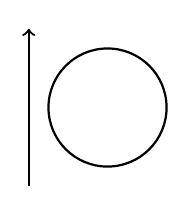
\begin{tikzpicture}
    \draw[thick] (0,0) circle (0.75);

    \draw[->, thick] (-1,-1) -- (-1,1);
\end{tikzpicture}
        \caption{$\Delta < 0$}
        \label{fig:sphere_hit_1}
    \end{subfigure}
    \begin{subfigure}[b]{0.27\textwidth}
        \centering
        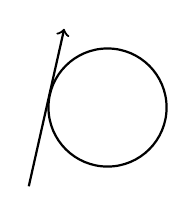
\begin{tikzpicture}
    \draw[thick] (0,0) circle (0.75);

    \draw[->, thick] (-1,-1) -- (-0.55,1);
\end{tikzpicture}
        \caption{$\Delta = 0$}
        \label{fig:sphere_hit_2}
    \end{subfigure}
    \begin{subfigure}[b]{0.27\textwidth}
        \centering
        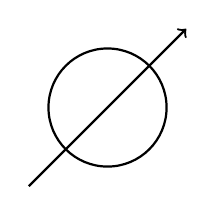
\begin{tikzpicture}
    \draw[thick] (0,0) circle (0.75);

    \draw[->, thick] (-1,-1) -- (1,1);
\end{tikzpicture}
        \caption{$\Delta > 0$}
        \label{fig:sphere_hit_3}
    \end{subfigure}
    \caption{Esquema de las tres posibilidades de determinante y su significado geométrico.}
    \label{fig:sphere_hit}
\end{figure}

Es únicamente este último caso el que se busca en la simulación, ya que un contacto tangencial no tiene relevancia física para el problema: el volumen de las esferas no corresponde de forma correcta con el de las antenas, por lo que en esos casos los rayos no impactarían de forma directa con la propia antena en un entorno real.
Por ello, solo se considerará la existencia de un impacto en el caso de que el discriminante de la Ec.~\eqref{eq:esfera_ti} sea estrictamente mayor que cero.

Es posible, por las mismas razones que se explicaban en el caso de los planos, que las soluciones tomen valores negativos.
De nuevo, no se considerarán estos casos como impactos de los rayos al no encontrarse en su dirección de propagación.

Se obtienen dos soluciones para $t_i$.
Si ambas son positivas, está claro que la solución en el caso de la suma en la Ec.~\eqref{eq:esfera_ti} será siempre mayor que la de la resta, por lo que es en este último caso en el que la distancia de impacto es menor.

Se tomará ese valor --el de la resta-- como solución final para determinar el punto de intersección de rayo y esfera, recurriendo de nuevo a la Ec.~\eqref{eq:recta_ti} para obtener sus coordenadas.

\subsubsection*{Determinación del ángulo de impacto}

Para simular de forma correcta el comportamiento de las antenas será necesario determinar el ángulo de impacto del rayo en los receptores, de la misma forma que se hacía en las paredes --aunque ahora no se busquen rayos reflejados--.

Para ello este caso es más sencillo.
Bastará con pasar a coordenadas esféricas la dirección del ángulo incidente, a las que se podrían añadir ciertos \textit{offsets} en cada uno de los ejes si los receptores se colocan con una orientación distinta a la de los ejes cartesianos.

% QUIZÁ ESTO NO VAYA AQUI.
% La elección de modelizar estos receptores como esferas parte de los múltiples rayos que impactarán sobre ellas.
% Al lanzar un gran número de rayos, todos los receptores recibirán varios --más aún con los sucesivos rebotes--, por lo que no podremos registrarlos todos.

% La elección correcta será la del rayo que impacte de forma más directa, ya que el resto de ellos serán residuos fruto del volumen de la esfera que no están presentes en la realidad.

% Es posible determinar este rayo teniendo en cuenta en el ángulo de incidencia respecto a la normal de la esfera, pero este paso es evitable teniendo en cuenta que el decaimiento de la potencia es función de la distancia recorrida.

\subsection{Electromagnetismo en los impactos}

Con las bases de la geometría del problema establecidas, resta abordar la física del problema: la interacción electromagnética de los rayos con el medio.

Como punto de partida es necesario abordar el comportamiento de estos rayos en su camino anterior a cualquier impacto contra alguno de los obstáculos, para lo que es habitual el uso de la ecuación de transmisión de Friis, definida como\cite{Antennas}
\begin{equation}
    \label{eq:Friis}
    P_t = P_i \left( \frac{\lambda}{4\pi r} \right)^2
\end{equation}
donde $P_t$ indica la potencia de una señal de longitud de onda $\lambda$ a una distancia $r$, siendo emitida en su origen por una potencia $P_i$.

Esta ecuación es una aproximación que no siempre es aplicable.
Su uso se limita a la modelización de la señal emitida y captada por antenas, en las que se omite cualquier efecto de reflexión entre ellas.

Para poder hacer esta consideración, se establece el límite
\begin{equation}
    r > \frac{2D^2}{\lambda}
\end{equation}
como rango válidos, con $D$ siendo el tamaño característico de las antenas --en el caso de que sean distintos, se considera el mayor de ellos--.

Teniendo en cuenta que en este caso se usarán ondas de WiFi de $2.4\si{\giga\hertz}$, su longitud de onda será $\lambda\approx 0.12\si{\meter}$.
Las antenas a usar tienen un tamaño de entre 10 y 20 cm, así que la Ec.~\eqref{eq:Friis} será valida a distancias superiores a unos 70cm.


\subsubsection*{Comportamiento tras los impactos}

Tras su recorrido libre en el aire, a su llegada al punto de impacto contra alguna de las paredes u obstáculos el rayo seguirá las leyes de Fresnel para la frontera entre dos medios.

En este caso son solo de interés las expresiones de los coeficientes de reflexión y transmisión de la potencia, que describen la proporción de energía de los rayos reflejados y transmitidos respectivamente.

Estas ecuaciones tendrán expresiones distintas dependiendo de si tratamos ondas s-polarizadas --con el campo eléctrico perpendicular al plano de incidencia-- o p-polarizadas --con el campo eléctrico paralelo al plano de incidencia--.\cite{5G_Simulation}
\begin{equation}
    \label{eq:coeff_reflx_1}
    \begin{aligned}
        R_\mathrm{s} &= \left|\frac{Z_2 \cos(\theta_i) - Z_1 \cos(\theta_t)}{Z_2 \cos(\theta_i) + Z_1 \cos(\theta_t)}\right|^2\\
        R_\mathrm{p} &= \left|\frac{Z_2 \cos(\theta_t) - Z_1 \cos(\theta_i)}{Z_2 \cos(\theta_t) + Z_1 \cos(\theta_i)}\right|^2
    \end{aligned}
\end{equation}
donde $Z_i$ hace referencia a la impedancia de la onda en cada medio, dada por
\begin{equation}
    Z = \sqrt{\frac{j\omega\mu}{\sigma + j\omega\varepsilon}}
\end{equation}
con $\mu$ indicando la permeabilidad magnética del medio, $\varepsilon$ la permivitidad dieléctrica y $\omega$ la frecuencia angular de la onda en cuestión.

Asumiendo que ambos medios son no magnéticos --es decir, $\mu = \mu_0$, como va a ser el caso en las simulaciones a realizar-- las expresiones de la Ec.~\eqref{eq:coeff_reflx_1} pasan a depender de los índices de refracción de modo que
\begin{equation}
    \label{eq:coeff_reflx_1}
    \begin{aligned}
        R_\mathrm{s} &= \left|\frac{n_1 \cos(\theta_i) - n_2\cos(\theta_t)}{n_1 \cos(\theta_i) + n_2\cos(\theta_t)}\right|^2\\
        R_\mathrm{p} &= \left|\frac{n_1 \cos(\theta_t) - n_2\cos(\theta_i)}{n_1 \cos(\theta_t) + n_2\cos(\theta_i)}\right|^2
    \end{aligned}
\end{equation}

Es posible eliminar el término dependiente del ángulo transmitido usando la ley de Snell de la refracción, de modo que las Ecs.\eqref{eq:coeff_reflx_1} pasan a ser
\begin{equation}
    \label{eq:coeff_reflx_2}
    \begin{aligned}
        R_\mathrm{s} &= \left|\frac{n_1 \cos(\theta_i) - n_2\sqrt{1 - \left[ \frac{n_1}{n_2}\sin(\theta_i)\right]^2}}{n_1 \cos(\theta_i) + n_2\sqrt{1 - \left[ \frac{n_1}{n_2}\sin(\theta_i)\right]^2}}\right|^2\\
        R_\mathrm{p} &= \left|\frac{n_1 \sqrt{1 - \left[ \frac{n_1}{n_2}\sin(\theta_i)\right]^2} - n_2\cos(\theta_i)}{n_1 \sqrt{1 - \left[ \frac{n_1}{n_2}\sin(\theta_i)\right]^2} + n_2\cos(\theta_i)}\right|^2
    \end{aligned}
\end{equation}

Asumiendo que el medio 1 es el aire, con índice de refracción igual a 1, se obtiene la expresión final usada en la simulación
\begin{equation}
    \label{eq:coeff_reflx_3}
    \begin{aligned}
        R_\mathrm{s} &= \left|\frac{\cos(\theta_i) - \sqrt{\varepsilon_r - \sin[2](\theta_i)}}{\cos(\theta_i) + \sqrt{\varepsilon_r - \sin[2](\theta_i)}}\right|^2\\
        R_\mathrm{p} &= \left|\frac{\varepsilon_r\cos(\theta_i) - \sqrt{\varepsilon_r - \sin[2](\theta_i)}}{\varepsilon_r\cos(\theta_i) + \sqrt{\varepsilon_r - \sin[2](\theta_i)}}\right|^2
    \end{aligned}
\end{equation}
donde se ha utilizado la relación $n = \sqrt{\varepsilon}$, dejando las expresiones dependiendo solo de la permitividad dieléctrica del medio y el ángulo de incidencia.

Para cada uno de los dos casos, la potencia transmitida será
\begin{equation}
    T_i = 1 - R_i
\end{equation}
por consevación de la energía.

Queda por aclarar la polarización de la ondas emitidas.
La aproximación tomada es asumir ondas no polarizadas, o lo que es lo mismo, con polarización circular, de modo que las energías de los campos eléctrico y magnético son las mismas y es posible tomar un coeficiente de reflexión de 
\begin{equation}
    R = \frac{1}{2} \left[ R_\mathrm{s} + R_\mathrm{p} \right]
\end{equation}

% Por último, también existirá en los rebotes un fenómeno de difración en el que se generan rayos de forma isotrópica.
% Aunque es un comportamieno que se incluye en algunos modelos de propagación en exteriores --donde las antenas direccionales tienen una potencia muy concentrada--, su efecto en interiores es despreciable, donde las potencias de emisión son mucho menores.

% Por ello, no se implementarán en este modelo.
% La potencia de cálculo extra requerida no compensa su contribución a los resultados, de modo que, al igual que en otros modelos de propagación interior, se considerará que no se produce.

% En la sección anterior se han sentado las bases geométricas para estudiar la propagación de los rayos, pero se ha obviado cualquier discursión sobre su interacción con las paredes u obstáculos, que obedecerá a leyes del electromagnetismo.

% Los impactos contra cualquiera de los obstáculos van a seguir las leyes de Fresnel, siendo

\subsubsection*{Difracción y \textit{scattering}}

Además de los rayos recibidos de forma directa y por el reflejo en los objetos existen otros dos fenómenos de generación de radiación en los impactos.

En primero de ellos es la difracción.
En el contacto de los rayos con los objetos se crearán conos de emisión de otros rayos, pero su modelización es muy complicada.

Los coeficientes de difracción no tienen una expresión tan sencilla y existen métodos desarrollados desde hace décadas para su modelización como la teoría geométrica de la difracción --GTD por su nombre en inglés-- y posteriormente la teoría uniforme de la difracción --UTD--.\cite{Compilation}

En ambos casos las potencias de los rayos difractados será muy baja.
En el caso de que los rayos originales tengan una potencia muy alta estos productos de la difracción tendrán un efecto menor.
En la propagación de interiores, donde las potencias son muy bajas, su efecto será residual.\cite{5G_Simulation}

En esta simulación no se considerará este efecto.
El alto coste computacional y la dificultad en la modelización no compensa el escaso efecto que tendrá comparado con el resto de rayos.
En general, esta ausencia está también presente en otros modelos de trazado de rayos.

Por otro lado también existe el fenómeno de \textit{scattering}, fruto de ciertas irregularidades y bordes en las superficies de los obstáculos y paredes.\cite{Compilation}

Los rayos producidos por este fenómeno tienen, como en el caso anterior, muy poca potencia.
Su parametrización es importante en entornos urbanos por la alta cantidad de edificios, pero en el caso de interiores no es tan relevante.

Por ello, por los mismos argumentos utilizados para los rayos difractados se aplican en este caso: el coste computacional no compensa el escaso efecto que producirían en los resultados, por lo que no se considerarán en la simulación.

\subsection{Antenas}
\label{sec:antenas}

Una vez establecidas las bases para la evaluación de los rayos en el área de interés es necesario abordar su origen y su recepción.

La emisión y recepción de estos rayos se hará mediante antenas que tendrán cierta direccionalidad fruto de su simetría que será necesario considerar.
Aquí aparece el concepto de direccionalidad, donde se parametriza la intensidad de la emisión o recepción dependiendo del ángulo de emisión o incidencia del ángulo.\cite{Antennas}

Esta directividad está definida como
\begin{equation}
    D = \frac{4\pi U}{P_\text{rad}}
\end{equation}
donde $U$ indica la potencia por unidad de ángulo sólido y $P_\text{rad}$ la potencia total emitida.

En el caso de la antena receptora se obtiene la misma expresión, teniendo en el denominador la potencia recibida.
Este valor de recepción es a veces llamado «ganancia», aunque su origen y concepto es el mismo que la direccionalidad.

En el caso de que una antena emita isotrópicamente la direccionalidad será la misma para todos los ángulos, de modo que es posible definir la direccionalidad como la razón entre la potencia de emisión entre la potencia de emisión si tuviese una emisión isotrópica.

La obtención de la función de forma general se obtiene de forma numérica.
En el caso de antenas con un diseño con alguna simetría existen expresiones analíticas, pero no podrán ser aplicadas en entornos reales como el que se trata en este trabajo.

Así, se recurrió a las utilidades proporcionadas en el \textit{Antenna Toolbox} de MATLAB, que permite definir antenas con un diseño arbitrario compuesta de una amplia serie de materiales y con ellos obtener su direccionalidad.\cite{MATLAB}

Las antenas utilizadas son antenas cilíndricas, como es habitual en el caso de comunicaciones WiFi.
En la Figura~\ref{fig:antenas} se incluyen dos imágnes de las antenas utilizadas.

\begin{figure}[H]
    \centering
    \begin{subfigure}[b]{0.45\textwidth}
        \centering
        \includegraphics[width=7cm]{pic/antena_router.jpg}
        \caption{Imágenes de la antena del router utilizado.}
        \label{fig:antena_router}
    \end{subfigure}
    \begin{subfigure}[b]{0.45\textwidth}
        \centering
        \includegraphics[width=7cm]{pic/antena_robot.jpg} 
        \caption{Imágenes de la antena receptora utilizada}
        \label{fig:antena_receptor}
    \end{subfigure}
    \caption{Imágenes de las antenas utilizadas.}
    \label{fig:antenas}
\end{figure}

En este caso se eligió una antena cilíndrica con $1\si{\milli\meter}$ de radio y $10\si{\centi\meter}$ de altura, con la alimentación justo a la mitad para componer una antena dipolar típica de cualquier router o receptor de WiFi.
Este modelo fue utilizado para las dos antenas utilizadas.

Esta antena forma un patrón con forma de toroide como se puede observar en la Figura~\ref{fig:patron_matlab}.
Así, se obtiene una direccionalidad algo mayor en ángulos cercanos al plano perpendicular al cilindro y prácticamente nula en el eje del propio cilindro.

La herramienta de MATLAB permite especificar los ángulos para los que se quiere generar valores de directividad al ser un cálculo numérico.
En este caso se generó con saltos de un ángulo sexagesimal, ya que permite un buen equilibrio entre una simulación que se completa en un tiempo razonable y puntos lo suficientemente juntos.
Para esta antena el patrón es muy suave, no es necesaria una precisión mayor.

\begin{figure}[H]
    \centering
    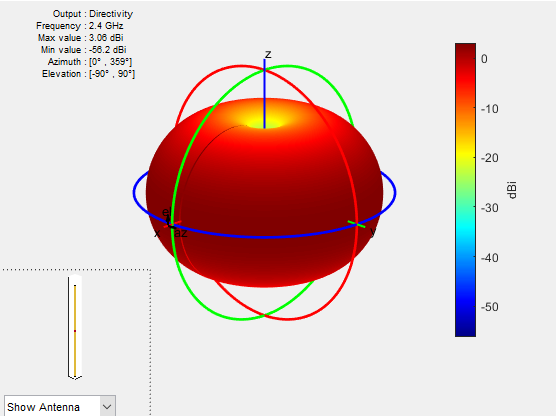
\includegraphics[width=0.6\textwidth]{pic/patron.png}
    \caption{Captura de la herramienta de MATLAB que permite visualizar el patrón de emisión numérico de una antena.}
    \label{fig:patron_matlab}
\end{figure}

Otra de las propiedades que proporciona esta herramienta es la de determinar la polarización de la antena a partir del campo magnético y eléctrico en varios puntos de la misma, de la misma forma que lo hacía para el patrón de emisión.\cite{MATLAB}

En la Figura~\ref{fig:eh_matlab} se puede observar el patrón de la antena simulada.
Se puede observar que en prácticamente en todas las zonas la polarización es circular --es decir, no está polarizada-- obteniendo intensidades similares en ambos campos.

\begin{figure}[H]
    \centering
    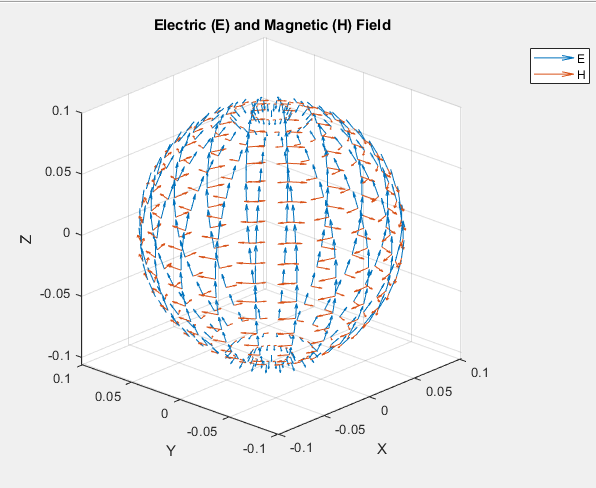
\includegraphics[width=0.6\textwidth]{pic/eh.png}
    \caption{Captura de la herramienta de MATLAB que permite visualizar la polarización de una antena.}
    \label{fig:eh_matlab}
\end{figure}

Esta polarización sí que cambia en zonas cercanas a la vertical de la antena, de la misma forma que ocurría con el patrón de emisión.

Esta característica es la que da pie a considerar rayos no polarizados en la sección anterior.
La antena solo emitirá ondas no polarizadas en las zonas con un patrón menor, es decir, donde la potencia de los rayos generados es menor.

Considerando el gran decaimiento de la potencia que sufren estos rayos con la distancia, el resto de rayos polarizados, con menor potencia en el origen, no tendrán un gran efecto respecto a los no polarizados.
Además, siendo generados prácticamente en la vertical de la antena, es poco probable que lleguen a los receptores, colocados mayoritamente a diferentes posiciones pero en el mismo plano.

